%% LaTeX Beamer presentation template (requires beamer package)
%% see http://bitbucket.org/rivanvx/beamer/wiki/Home
%% idea contributed by H. Turgut Uyar
%% template based on a template by Till Tantau
%% this template is still evolving - it might differ in future releases!

%% Template edited by Panagiotis Adamopoulos {padamopo}@stern.nyu.edu

\documentclass{beamer}

\mode<presentation>
{
\usetheme{NYU}

\setbeamercovered{transparent}
}


\usepackage[english]{babel}
\usepackage[latin1]{inputenc}
\usepackage{subfigure}
\usepackage{pgfplots}
% font definitions, try \usepackage{ae} instead of the following
% three lines if you don't like this look
\usepackage{mathptmx}
\usepackage[scaled=.90]{helvet}
\usepackage{courier}
\usepackage{graphicx}
\graphicspath{{pics/}}
\usepackage{listings}
\lstset{numbers=left,
 numberstyle= \tiny,
 keywordstyle= \color{blue!70},commentstyle=\color{red!50!green!50!blue!50},
 frame=shadowbox,
 rulesepcolor= \color{red!20!green!20!blue!20},
 xleftmargin=2em
 }
\usepackage{xcolor}
\usepackage{extarrows}
\usepackage{array}
\usepackage{verbatim}
\usepackage{hyperref}
\usepackage{tikz}
\usepackage{tikz-qtree}

\usepackage[T1]{fontenc}


\usepackage{comment}
%usepackage{appendixnumberbeamer}
%\usepackage{amsmath}
\usepackage{pgfpages}

\usetikzlibrary{calc}
\newcounter{nodeidx}
\setcounter{nodeidx}{1}
\newcommand{\nodes}[1]{%
    \foreach \num in {#1}{
      \node[minimum size=6mm, draw, rectangle] (\arabic{nodeidx}) at (\arabic{nodeidx},0) {\num};
      \stepcounter{nodeidx}
    }
}
\newcommand{\brckt}[4]{% from, to, lvl, text
  \draw (#1.south west) ++($(-.1, -.1) + (-.1*#3, 0)$) -- ++($(0,-.1) + (0,-#3*1.25em)$) -- node [below] {#4} ($(#2.south east) + (.1,-.1) + (.1*#3, 0) + (0,-.1) + (0,-#3*1.25em)$) -- ++($(0,#3*1.25em) + (0,.1)$);%
}

\title{Music Composition with RNN}

\subtitle{A Modern Approach}
\author{Wenliang~Zhao, Zhiyu~Feng, Qi~Feng}

% - Use the \inst command only if there are several affiliations.
% - Keep it simple, no one is interested in your street address.
\institute[NYU]
{
Department of Computer Science, Courant Institute of Mathematical Sciences\\
   \texttt{wz927}, \texttt{zf499}, \texttt{qf264@nyu.edu}
}

\date{December 06, 2016}


% This is only inserted into the PDF information catalog. Can be left
% out.
\subject{}

\begin{document}

\begin{frame}
\titlepage
\end{frame}

%\begin{frame}
%\frametitle{Outline}
%\tableofcontents
%\end{frame}

\section{The Problem}
\begin{frame}{The Music Generation Problem}
Can we use machine learning to create compelling art and music?
\end{frame}
\begin{frame}{WER Assignment}
  \begin{itemize}
    \item
    Language modeling -- connections among tokens in a sequence.
    \item
    Perplexity as an evaluation measure.
  \end{itemize}
\end{frame}

\begin{frame}{Difference Between Music and Language}
  \begin{itemize}
    \item
    Tempo.
    \item
    Multitrack.
    \item
    Long repetition.
    \item
    Harmony (Already solved in Baseline Model).
  \end{itemize}
\end{frame}

\begin{frame}{Baseline}
Baseline model used in this project is a LSTM RNN model implemented by Yoav Zimmerman.
\begin{itemize}
  \item
  Music have two seperated parts: a melody and harmony.
  Melody allows at most one note playing at every time step.
  Harmony allows more than one note to be played at each time step.
  \item
  All harmony can be classified into a chord class. Ex: a C, E, G active during a time step can be classified as a C Major.
\end{itemize}
\end{frame}

\begin{frame}{Model}
	\begin{center}
	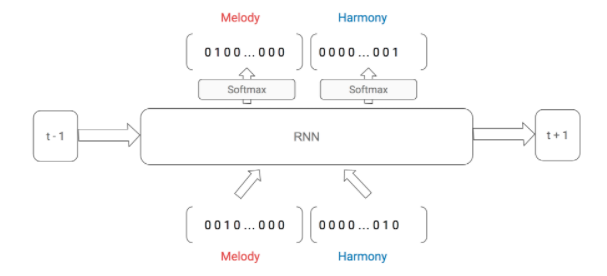
\includegraphics[scale=0.4]{baseline_model}
	\end{center}
\small \[L(z, m, h) =  \alpha \, log \bigg( \frac{ e^{z_m} }{ \sum_{n=0}^{M-1}{ e^{z_n}}} \bigg) + (1 - \alpha) \, log \bigg( \frac{ e^{z_{M+h}} }{ \sum_{n=M}^{M+H}{ e^{z_n}}} \bigg)\]
\begin{itemize}
	\item
	\small M,H: number of melody and  harmony classes
	\item
	\small m,h: target melody and harmony classes
	\item 
	\small $\alpha$: melody coeffcient 
\end{itemize}
\end{frame}

\section{Baseline}
\begin{frame}{Model Performance} 
  \begin{center} 
  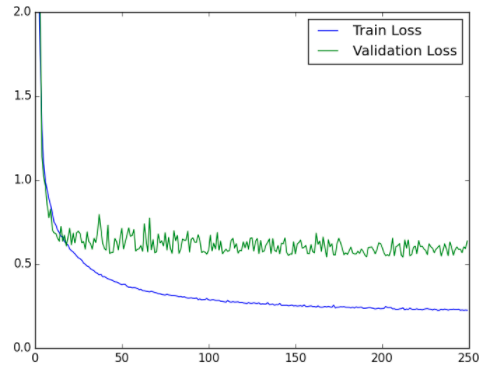
\includegraphics[scale=0.3]{baseline_performance} 
  \end{center} 
\small \[L(z, m, h) =  \alpha \, log \bigg( \frac{ e^{z_m} }{ \sum_{n=0}^{M-1}{ e^{z_n}}} \bigg) + (1 - \alpha) \, log \bigg( \frac{ e^{z_{M+h}} }{ \sum_{n=M}^{M+H}{ e^{z_n}}} \bigg)\] 
\begin{itemize} 
  \item 
  \small M,H: number of melody and  harmony classes 
  \item 
  \small m,h: target melody and harmony classes 
  \item 
  \small $\alpha$: melody coeffcient 
\end{itemize}
\end{frame}

\section{Learning Framework}

\begin{frame}{Distinguishing Different Tempo}
  \begin{itemize}
    \item
    Record information from previous time step.
    \begin{itemize}
      \item If the note was played?
      \item If the note was played by holding?
    \end{itemize}
  \end{itemize}

  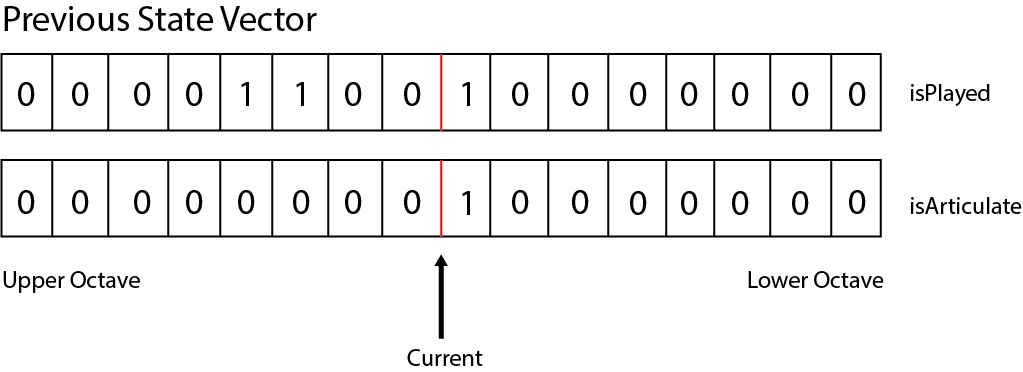
\includegraphics[scale=0.3]{previous_state.jpg}
\end{frame}

\begin{frame}{Multi-Track Music}
    Using multiple vectors presenting all tracks 
    \newline

    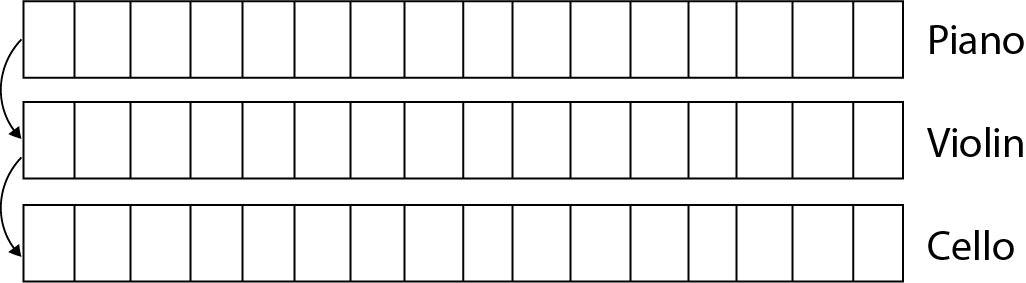
\includegraphics[scale=0.3]{multi-track.jpg}
\end{frame}

\begin{frame}{Keeping Long Term Memory}
  \begin{itemize}
    \item
    Hierachical RNN.
  \end{itemize}
  \begin{center}
  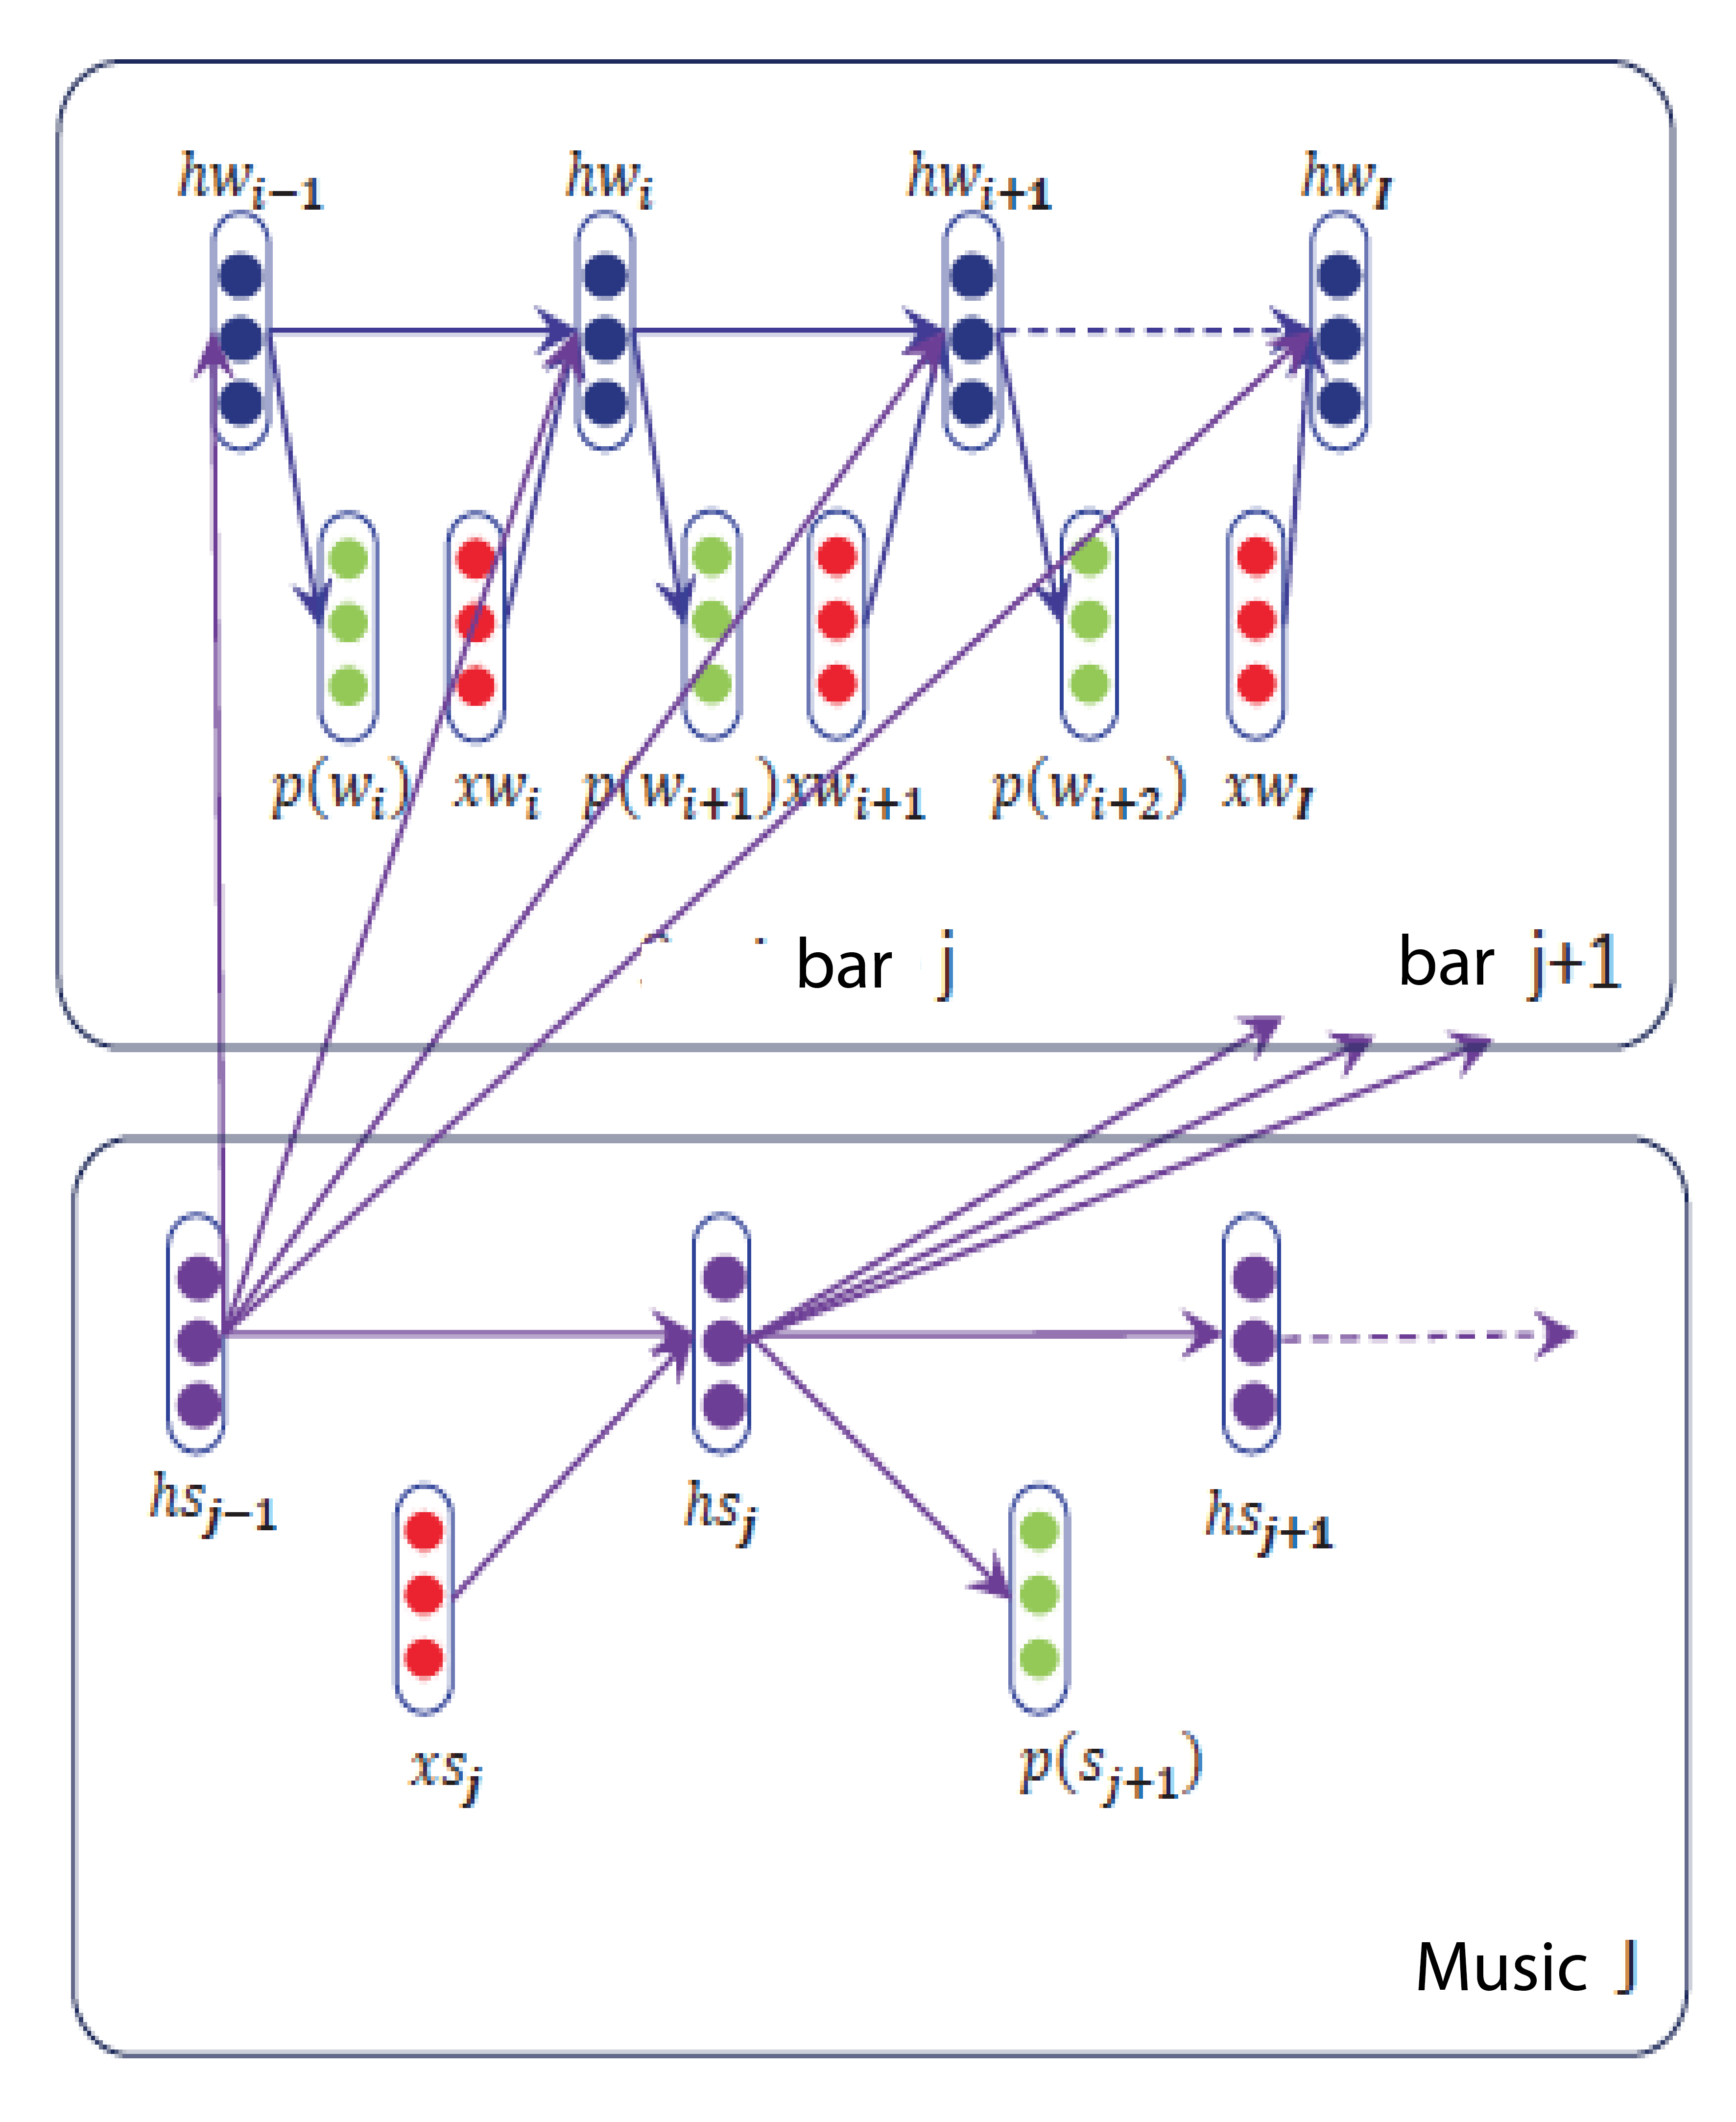
\includegraphics[scale=0.1]{hierarchical1.png}
  \end{center}
\end{frame}

\begin{frame}{Two types of Learning Problem}
  \begin{itemize}
    \item Generate original music pieces.
    \item Give several consecutive bars. Predict the next bars.
  \end{itemize}
\end{frame}

\begin{frame}{Evaluation}
  \begin{itemize}
    \item Turing test.
    \item Prediction Accuracy on test set.
  \end{itemize}
\end{frame}

\begin{frame}{Datasets}
\begin{itemize}
\item
Piano-midi.de: classical piano pieces. (http://www.piano-midi.de/)
\item
Nottingham: over 1000 folk tunes.
\end{itemize}
\end{frame}

\begin{frame}{Q\&A}
  Questions?
\end{frame}

\end{document}
